\documentclass[aspectratio=169]{beamer}
\usepackage{ITMOtheme}
\usepackage{amsmath}
\usepackage{amssymb}
\usepackage{graphicx} % For including images if needed
\usepackage{amsfonts} % For \mathbb symbols
% pt produsu cartezian
\usepackage{mathabx}
\usepackage{mathtools}

% If ITMOtheme is not used, define some colors for consistency or use standard beamer colors
% \definecolor{ITMOblue}{RGB}{0,70,132}
% \definecolor{ITMOred}{RGB}{200,0,0}

\title[Hopf Bifurcations in CRNs]{Proving existence and ruling out of Hopf bifurcations in Phosphorylation–Dephosphorylation reaction networks}
\author{Stan Ioan-Victor}
\date{\today}
\institute{UBB MIE3}

\begin{document}

\begin{frame}[plain]
	\titlepage
\end{frame}

\begin{frame}{Outline}
	\tableofcontents
\end{frame}

% --- Section 1: Why Study Chemical Rhythms? ---
\section{Why Study Chemical Rhythms?}

\begin{frame}{\insertsectionhead}
	\frametitle{The Importance of Biological Oscillations}
	\begin{itemize}
		\item Many biological processes are not static; they \alert{oscillate} or cycle over time. Think of:
			\begin{itemize}
				\item \textbf{Circadian Rhythms:} Our internal 24-hour body clocks regulating sleep-wake cycles, hormone release, and metabolism.
				\item \textbf{Heartbeat \& Respiration:} Essential life-sustaining rhythmic activities.
				\item \textbf{Cell Cycle:} The ordered series of events leading to cell division and duplication.
				\item \textbf{Hormonal Cycles:} Regular fluctuations in hormone levels (e.g., menstrual cycle).
			\end{itemize}
		\item These rhythms are often driven by complex networks of interacting molecules - \alert{Chemical Reaction Networks (CRNs)}.
		\item Understanding how these networks generate oscillations is crucial to understanding life's phenomena.
	\end{itemize}
\end{frame}

\begin{frame}{\insertsectionhead}
	\frametitle{Phosphorylation: A Key Regulator \& Its Rhythms}
	\begin{itemize}
		\item \alert{Phosphorylation} (adding a phosphate group to a protein) and \alert{dephosphorylation} (removing it) are like molecular on/off switches.
		\item They are fundamental to \alert{cellular communication (signal transduction)}, controlling a vast array of cellular processes:
			\begin{itemize}
				\item Growth, development, and division.
				\item Responses to environmental cues.
				\item Immune responses.
			\end{itemize}
		\item \alert{Dysregulation} in these signaling pathways and their rhythms is implicated in many diseases:
			\begin{itemize}
				\item Cancer (uncontrolled cell growth).
				\item Diabetes (problems with insulin signaling).
				\item Neurological disorders.
				\item Inflammatory diseases.
			\end{itemize}
		\item Studying \alert{Hopf bifurcations} in these (de)phosphorylation CRNs helps us understand how these systems can switch from stable states to oscillatory behavior, providing insights into both normal function and disease mechanisms.
	\end{itemize}
\end{frame}

% --- Section 2: Introduction to Chemical Reaction Networks (CRNs) ---
\section{Introduction to Chemical Reaction Networks (CRNs)}

\begin{frame}{\insertsectionhead}
	\frametitle{What is a Chemical Reaction Network (CRN)?}
	A CRN consists of:
	\begin{itemize}
		\item A set of $\left|S\right| = n$ chemical \alert{species} $S = \{X_1, \dots, X_n\}$.
		\item A set of $r$ \alert{reactions}, each of the form:
			\[
				\alpha_{1j} X_1 + \dots + \alpha_{n j} X_n \xrightarrow{k_j} \beta_{1j} X_1 + \dots + \beta_{n j}, \forall j = \overline{1,r}.	
			\]
		\item $\alpha_{ij}, \beta_{ij} \in \mathbb{N}$ are \alert{stoichiometric coefficients} (stoichiometries) of reactants, respectively products.
		\item $k_j > 0$ are the \alert{reaction rate constants}.
		\item Concentrations are $x = (x_1, \dots, x_n)^T$, where $x_i = [X_i]$.
	\end{itemize}
\end{frame}

\begin{frame}{\insertsectionhead}
	\frametitle{Mass-Action Kinetics \& ODE Model}
	\begin{itemize}
		\item The \alert{rate} of a certain reaction $j$ (mass-action):
			$$ 	v_j : \mathbb{R}^r_{> 0} \bigtimes \mathbb{R}^n_{\geq 0} \rightarrow \mathbb{R}_{\geq 0}   $$
			$$ v_j(k,x) = k_j \prod_{i=1}^{n} x_i^{\alpha_{ij}} $$

		\item The \alert{flux vector} $v : \mathbb{R}^r_{> 0}  \bigtimes \mathbb{R}^n_{\geq 0} \rightarrow \mathbb{R}^r_{\geq 0}$:
			$$ 	(v(x,k))_{i} = v_i(k_i, x)$$
		\item The \alert{left / right stoichiometric matrices} $		\Gamma_L, \Gamma_R \in \mathcal{M}_{n \bigtimes r}(\mathbb{N}), 		(\Gamma_L)_{ij} = \alpha_{ij};
			(\Gamma_R)_{ij} = \beta{ij} $
		\item The \alert{stoichiometric matrix} $\Gamma \in \mathcal{M}_{n \times r}(\mathbb{Z})$: $\Gamma_{ij} = \beta_{ij} - \alpha_{ij}$ (net change).

	\end{itemize}
\end{frame}

% --- Section 3: Dynamical Systems Fundamentals ---
\section{Dynamical Systems Fundamentals}

\begin{frame}
	\begin{itemize}
		\item Dynamics via Ordinary Differential Equations (ODEs):
			$$ \frac{dx}{dt} = \Gamma \cdot v(k,x) $$
			This system models how concentrations change over time.

			Take this \textbf{open network} as an example:
	\end{itemize}
	\begin{align*}
		A + C \xrightarrow{k_{1}} 2A \\
		B + C \xrightarrow{k_{2}} 2B  \\
		A \xrightarrow{k_{3}} \emptyset \\
		B \xrightarrow{k_{4}} \emptyset \\
		\emptyset \xrightarrow{k_{5}} C
	\end{align*}
\end{frame}

\begin{frame}
	The stoichiometric matrices:
	\begin{align*}
		\Gamma_L =
		\begin{pmatrix}
			1 & 0 & 1 & 0 & 0 \\
			0 & 1 & 0 & 1 & 0 \\
			1 & 1 & 0 & 0 & 0
		\end{pmatrix}
		, \quad
		\Gamma_R =
		\begin{pmatrix}
			2 & 0 & 0 & 0 & 0 \\
			0 & 2 & 0 & 0 & 0 \\
			0 & 0 & 0 & 0 & 1
		\end{pmatrix}
	\end{align*}
	\begin{equation*}
		\Gamma =
		\begin{pmatrix*}
			1 & 0 & -1 & 0 & 0 \\
			0 & 1 & 0 & -1 & 0 \\
			-1 & -1 & 0 & 0 & 1
		\end{pmatrix*}
	\end{equation*}
	Whereas, the reaction rate (\textbf{flux vector}):
	\[
		v(k,x) =
		\begin{pmatrix*}
			v_{1}(k,x)	 \\
			v_{2}(k,x)	 \\
			v_{3}(k,x)	 \\
			v_{4}(k,x)	 \\
			v_{5}(k,x)
		\end{pmatrix*} =
		\begin{pmatrix}
			k_1 x_1 x_3 \\
			k_2 x_2 x_3 \\
			k_3 x_1 \\
			k_4 x_2 \\
			k_5
		\end{pmatrix}
	\]
\end{frame}

\begin{frame}
	And so its dynamical system in matrix form is:
	\begin{align*}
		\frac{dx}{dt} &= \Gamma v(k,x) \\
		\frac{d}{dt}
		\begin{pmatrix*}
			x_1	\\
			x_2	\\
			x_3	
		\end{pmatrix*} &=
		\begin{pmatrix*}
			1 & 0 & -1 & 0 & 0 \\
			0 & 1 & 0 & -1 & 0 \\
			-1 & -1 & 0 & 0 & 1
		\end{pmatrix*}
		\begin{pmatrix}
			k_1 x_1 x_3 \\
			k_2 x_2 x_3 \\
			k_3 x_1 \\
			k_4 x_2 \\
			k_5
		\end{pmatrix}
	\end{align*}
	Resulting in the ODE system:
	\[
		\begin{cases*}
			\dot{x}_1 = k_1 x_1 x_3 - k_3x_1  \\
			\dot{x}_2 = k_2 x_2 x_3 - k_4 x_2  \\
			\dot{x}_3 = -k_1 x_1 x_3 - k_2 x_2 x_3 + k_5 \\
		\end{cases*}
	\]
\end{frame}

\begin{frame}{\insertsectionhead}
	\frametitle{Ordinary Differential Equations (ODEs)}
	\begin{itemize}
		\item An ODE describes a function of one variable in terms of its derivatives. General form:
			$$ F(t, y(t), y'(t), \dots, y^{(n)}(t)) = 0 $$
		\item \alert{Explicit form}: $y^{(n)}(t) = f(t, y(t), \dots, y^{(n-1)}(t))$.
		\item A \alert{system of first-order ODEs}:
			$$ \dot{y}_i = f_i(t, y_1, \dots, y_n), \quad i=\overline{1, n} $$
			Vector form: $\dot{y} = f(t,y)$.
		\item CRN models are typically systems of first-order \alert{autonomous} ODEs.
	\end{itemize}	
\end{frame}

\begin{frame}{\insertsectionhead}
	\frametitle{Dynamical Systems: State, Flow, Orbits}
	A dynamical system $(T, S, \Phi)$ involves:
	\begin{itemize}
		\item $T$: Time (e.g., $\mathbb{R}_{\ge 0}$).
		\item $S$: State space (e.g., possible concentrations, $\mathbb{R}^n_{>0}$).
		\item $\Phi$: Evolution function $\Phi(t, s_0)$ gives the state at time $t$ starting from $s_0$.
			\begin{itemize}
				\item $\Phi(0, s) = s$.
				\item $\Phi(t_2, \Phi(t_1, s)) = \Phi(t_1+t_2, s)$.
			\end{itemize}
		\item The \alert{flow} through $s_0$ is $\Phi_{s_0}(t) = \Phi(t,s_0)$.
		\item The \alert{orbit} (or trajectory) $\gamma_{s_0}$ is the image of the flow: $\{\Phi(t,s_0) | t \in T\}$.
		\item An \alert{invariant set} $\mathcal{M} \subseteq S$ is s.t. $\forall s_0 \in \mathcal{M} \implies \Phi(t,s_0) \in \mathcal{M}, \forall t \ge 0$.
	\end{itemize}
\end{frame}

\begin{frame}
	\centering
	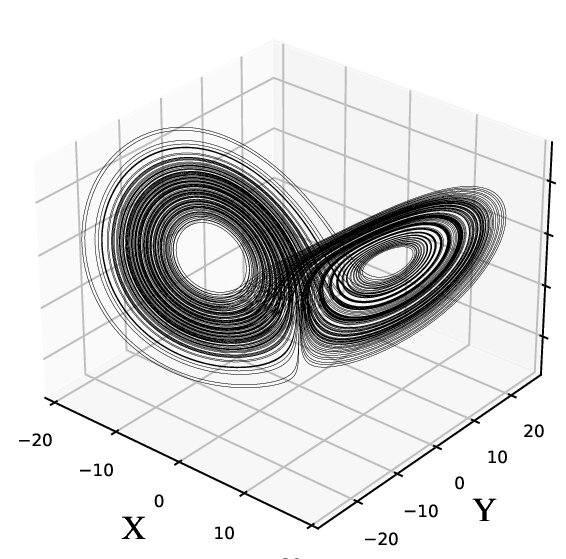
\includegraphics[width=0.6\linewidth]{pics/lorenz.jpg}\\
\end{frame}

\begin{frame}{\insertsectionhead}
	\frametitle{Equilibrium Points and Their Stability}
	For $\dot{x} = f(x)$:
	\begin{itemize}
		\item An \alert{equilibrium point} (steady state) $x^*$ satisfies $f(x^*) = 0$. The system remains at $x^*$ if started there.
			For a CRN: $\Gamma v(k, x^*) = 0$.
		\item \alert{Lyapunov Stability}: $x^*$ is stable if solutions starting close to $x^*$ stay close for all future time.
		\item \alert{Asymptotic Stability}: $x^*$ is asymptotically stable if it's Lyapunov stable AND solutions starting sufficiently close to $x^*$ converge to $x^*$ as $t \to \infty$. These are often called \alert{attractors}.
		\item \alert{Unstable}: If not stable. Solutions may diverge.
	\end{itemize}
\end{frame}

\begin{frame}{\insertsectionhead}
	\frametitle{Linearization and Eigenvalues}
	To analyze stability near an equilibrium $x^*$:
	\begin{itemize}
		\item \alert{Linearize} $\dot{x}=f(x)$ around $x^*$: Let $z = x - x^*$. Then $\dot{z} \approx J z$.
		\item The \alert{Jacobian matrix} $J$ at $x^*$: $J_{ij} = \frac{\partial f_i}{\partial x_j} \bigg|_{x^*}$.
		\item \alert{Eigenvalues $\lambda_k$} of $J$ dictate local behavior:
			\begin{itemize}
				\item All Re($\lambda_k$) $< 0 \implies x^*$ is asymptotically stable.
				\item Some Re($\lambda_k$) $> 0 \implies x^*$ is unstable.
				\item Some Re($\lambda_k$) $= 0$ (others $<0$) $\implies x^*$ is non-hyperbolic. \alert{Crucial for bifurcations!} (pretty hard to study given only the linearization).
			\end{itemize}
	\end{itemize}
\end{frame}

% --- Section 4: Bifurcation Theory ---
\section{Bifurcation Theory}

\begin{frame}{\insertsectionhead}
	\frametitle{What is a Bifurcation?}
	\begin{itemize}
		\item Consider $\dot{x} = f(x, \mu)$, where $\mu$ is a \alert{bifurcation parameter} (e.g., a rate constant, total amount of an enzyme).
		\item A \alert{bifurcation} occurs at $\mu_0$ if the system's qualitative behavior changes as $\mu$ passes $\mu_0$.
		\item Examples of changes:
			\begin{itemize}
				\item Number or stability of equilibria.
				\item Appearance/disappearance of \alert{periodic orbits (limit cycles)}.
			\end{itemize}
		\item \alert{Local bifurcations} involve changes near an equilibrium and are detected via Jacobian eigenvalues.
		\item Whereas \alert{global bifurcations} involve changes in the system's topology or structure, often requiring more complex analysis.
	\end{itemize}
\end{frame}

\begin{frame}{\insertsectionhead}
	\frametitle{Common Local Bifurcations (1D context for intuition)}
	For $\dot{y} = f(y, \mu)$ with $f(0,0)=0, \frac{\partial f}{\partial y}(0,0)=0$:
	\begin{itemize}
		\item \alert{Saddle-Node}: Two equilibria collide and annihilate (or are born). Requires $\frac{\partial f}{\partial \mu} \neq 0, \frac{\partial^2 f}{\partial y^2} \neq 0$.
		\item \alert{Transcritical}: An equilibrium exists for all $\mu$ but exchanges stability with another equilibrium that crosses it. Requires $\frac{\partial^2 f}{\partial \mu \partial y} \neq 0, \frac{\partial^2 f}{\partial y^2} \neq 0$.
		\item \alert{Pitchfork}: One equilibrium splits into three (or vice-versa), often due to symmetry. Requires $f(-y,\mu)=-f(y,\mu)$, $\frac{\partial^2 f}{\partial \mu \partial y} \neq 0, \frac{\partial^3 f}{\partial y^3} \neq 0$.
	\end{itemize}
	These illustrate how parameter changes can alter system structure. Our focus is on a bifurcation that creates oscillations in higher dimensions: the Hopf Bifurcation.
\end{frame}

\begin{frame}
	\centering
	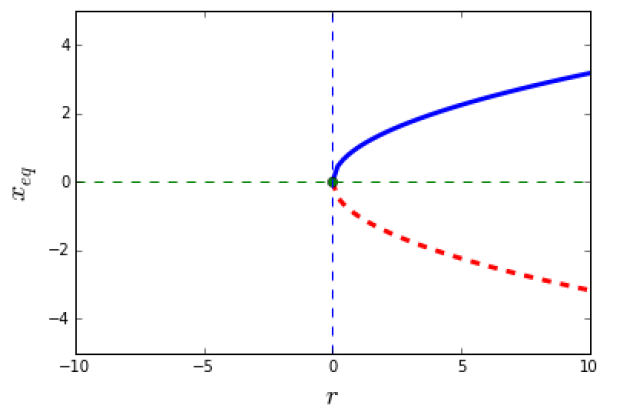
\includegraphics[width=0.8\linewidth]{pics/saddle-node-bif.png}\\
	\tiny (Illustrative: Saddle-node bifurcation)
\end{frame}

\begin{frame}
	\centering
	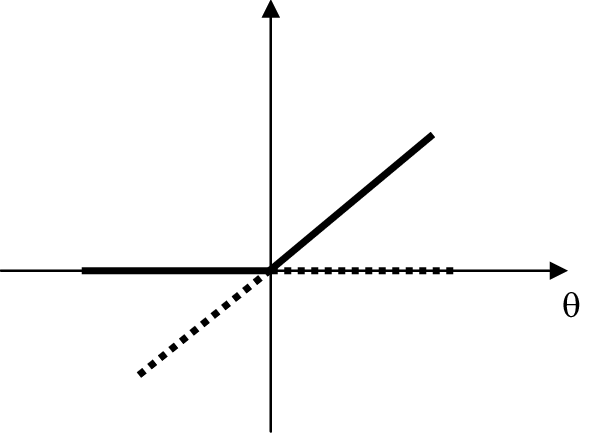
\includegraphics[width=0.8\linewidth]{pics/transcritical-bif.png}\\
	\tiny (Illustrative: Transcritical bifurcation)
\end{frame}

\begin{frame}
	\centering
	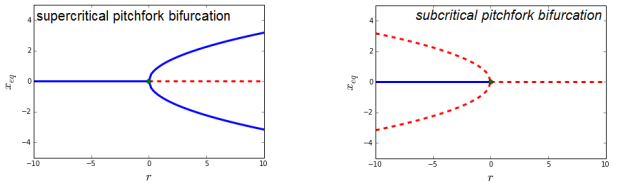
\includegraphics[width=1.01\linewidth]{pics/pitchfork-bif.png}\\
	\tiny (Illustrative: Pitchfork bifurcation)
\end{frame}

\begin{frame}{\insertsectionhead}
	\frametitle{Hopf Bifurcation: The Birth of Oscillations}
	A simple Hopf bifurcation occurs at $(x^*, \mu_0)$ if:
	\begin{enumerate}
		\item $J(x^*, \mu_0)$ has a \alert{single pair of complex conjugate eigenvalues} $\lambda_{1,2}(\mu) = \alpha(\mu) \pm i\omega(\mu)$ with:
			\begin{itemize}
				\item $\alpha(\mu_0) = 0$ (purely imaginary at $\mu_0$).
				\item $\omega(\mu_0) \neq 0$ (non-zero frequency).
			\end{itemize}
		\item All other $n-2$ eigenvalues have Re($\lambda_j$) $< 0$.
		\item \alert{Transversality}: $\frac{d\alpha}{d\mu}\bigg|_{\mu_0} \neq 0$ (eigenvalues cross imaginary axis with non-zero speed).
	\end{enumerate}
	\alert{Result}: A stable equilibrium can lose stability, giving rise to a stable \alert{limit cycle} (sustained oscillation), or an unstable one can become stable.
\end{frame}

\begin{frame}{\insertsectionhead}
	\frametitle{Limit Cycles}
	\begin{itemize}
		\item A \alert{closed orbit (or cycle)} $\gamma$ is an orbit that is periodic: $\Phi(t+T, s_0) = \Phi(t, s_0)$ for some period $T>0$ and $\forall s_0 \in \gamma$.
		\item A \alert{limit cycle} is an isolated closed orbit. Solutions nearby either spiral towards it (stable limit cycle) or away from it (unstable limit cycle).
		\item \textbf{Poincaré-Bendixson Theorem (for 2D systems):} for a system in $X \subseteq \mathbb{R}^2, \forall S$ compact invariant set without equilibria $\implies \forall s \in S$ either tend to limit cycles, or are limit cycles themselves. (This doesn't directly apply to $n>2$ dimensions, but Hopf gives a mechanism for limit cycles in $\mathbb{R}^n$).
		\item Hopf bifurcations are a primary mechanism for the creation of limit cycles from equilibria.
	\end{itemize}
\end{frame}

\begin{frame}{\insertsectionhead}
	\frametitle{Visualizing a Supercritical Hopf Bifurcation}
	As parameter $\mu$ increases through $\mu_0$:
	\begin{columns}[T]
		\column{0.5\textwidth}
		\textbf{Eigenvalue Movement:}
		\begin{itemize}
			\item $\mu < \mu_0$: Re($\lambda_{1,2}$) < 0 (stable focus)
			\item $\mu = \mu_0$: Re($\lambda_{1,2}$) = 0 (center-like)
			\item $\mu > \mu_0$: Re($\lambda_{1,2}$) > 0 (unstable focus)
		\end{itemize}
		\centering
		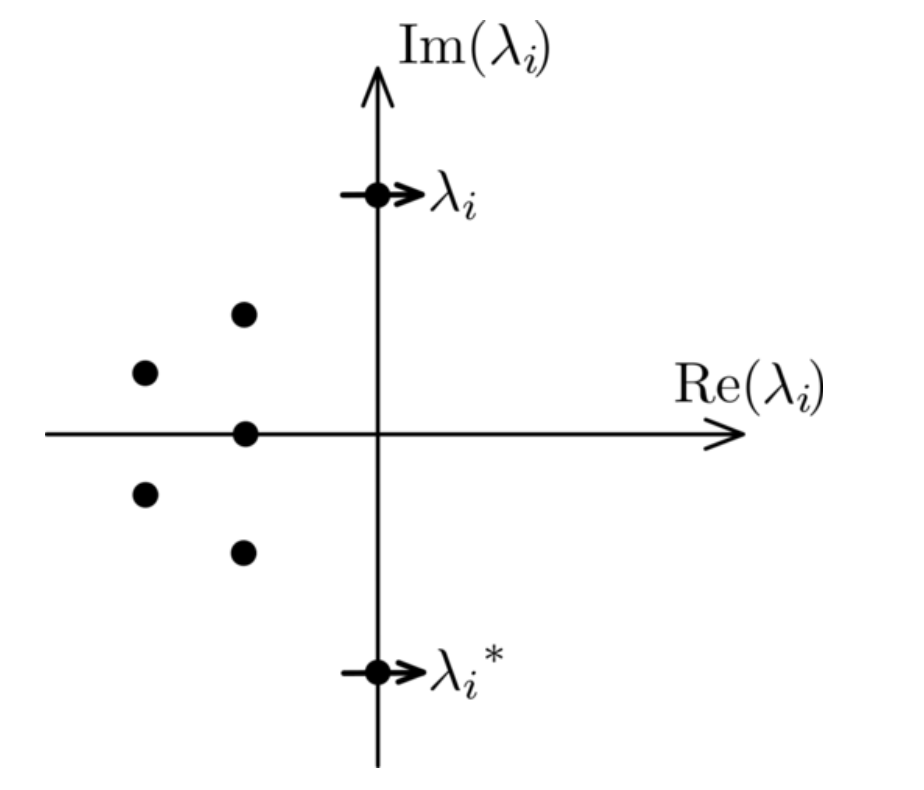
\includegraphics[width=0.8\linewidth]{pics/hopf-bif-eigenvalue-graph.png}\\
		\tiny (Illustrative: Eigenvalues crossing imaginary axis)

		\column{0.5\textwidth}
		\textbf{Phase Portrait Change:}
		\begin{itemize}
			\item $\mu < \mu_0$: Stable equilibrium.
			\item $\mu > \mu_0$: Equilibrium unstable, stable limit cycle appears.
		\end{itemize}
		\centering
		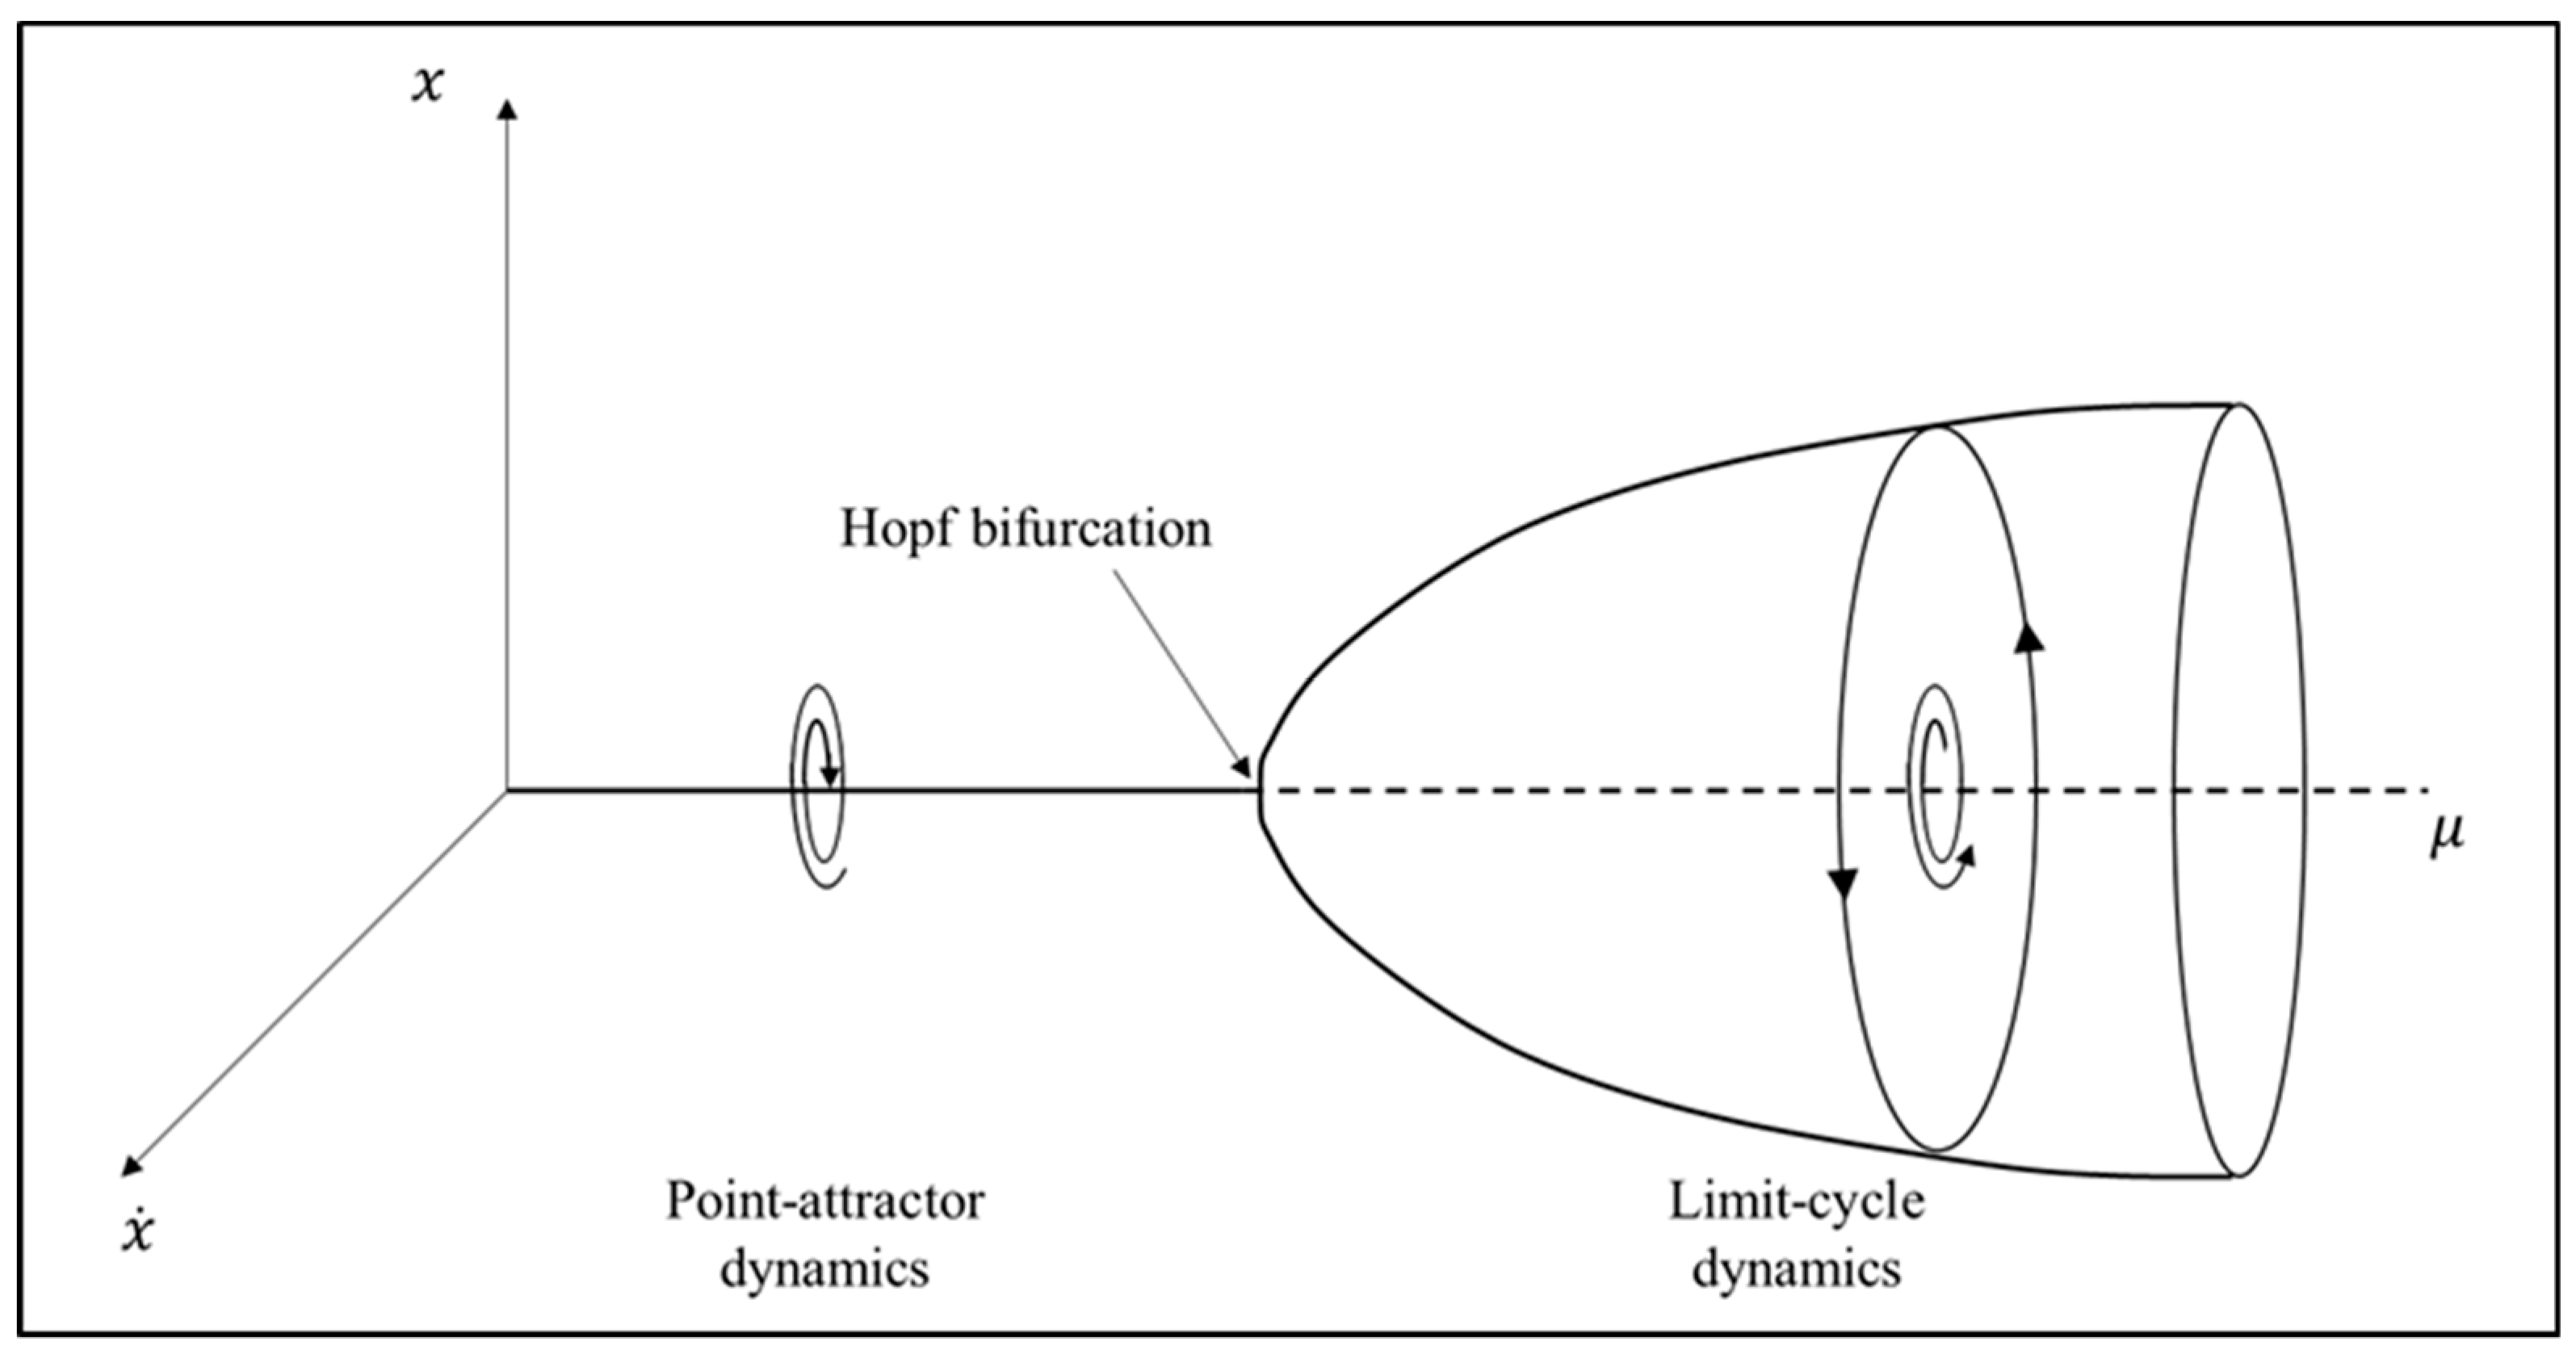
\includegraphics[width=0.8\linewidth]{pics/hopf-bif-pic.png}\\
		\tiny (Illustrative: Birth of a limit cycle)
	\end{columns}
	\vspace{0.5cm}
	\small Supercritical: stable limit cycle born. Subcritical: unstable limit cycle merges/destroys stable equilibrium.
\end{frame}

\begin{frame}
	So having these in mind, Hopf is kind of like an $\mathbb{R}^n$ version of a Pitchfork bifurcation when you think about it.
	You can even see the resemblance in the way they look
	\centering
	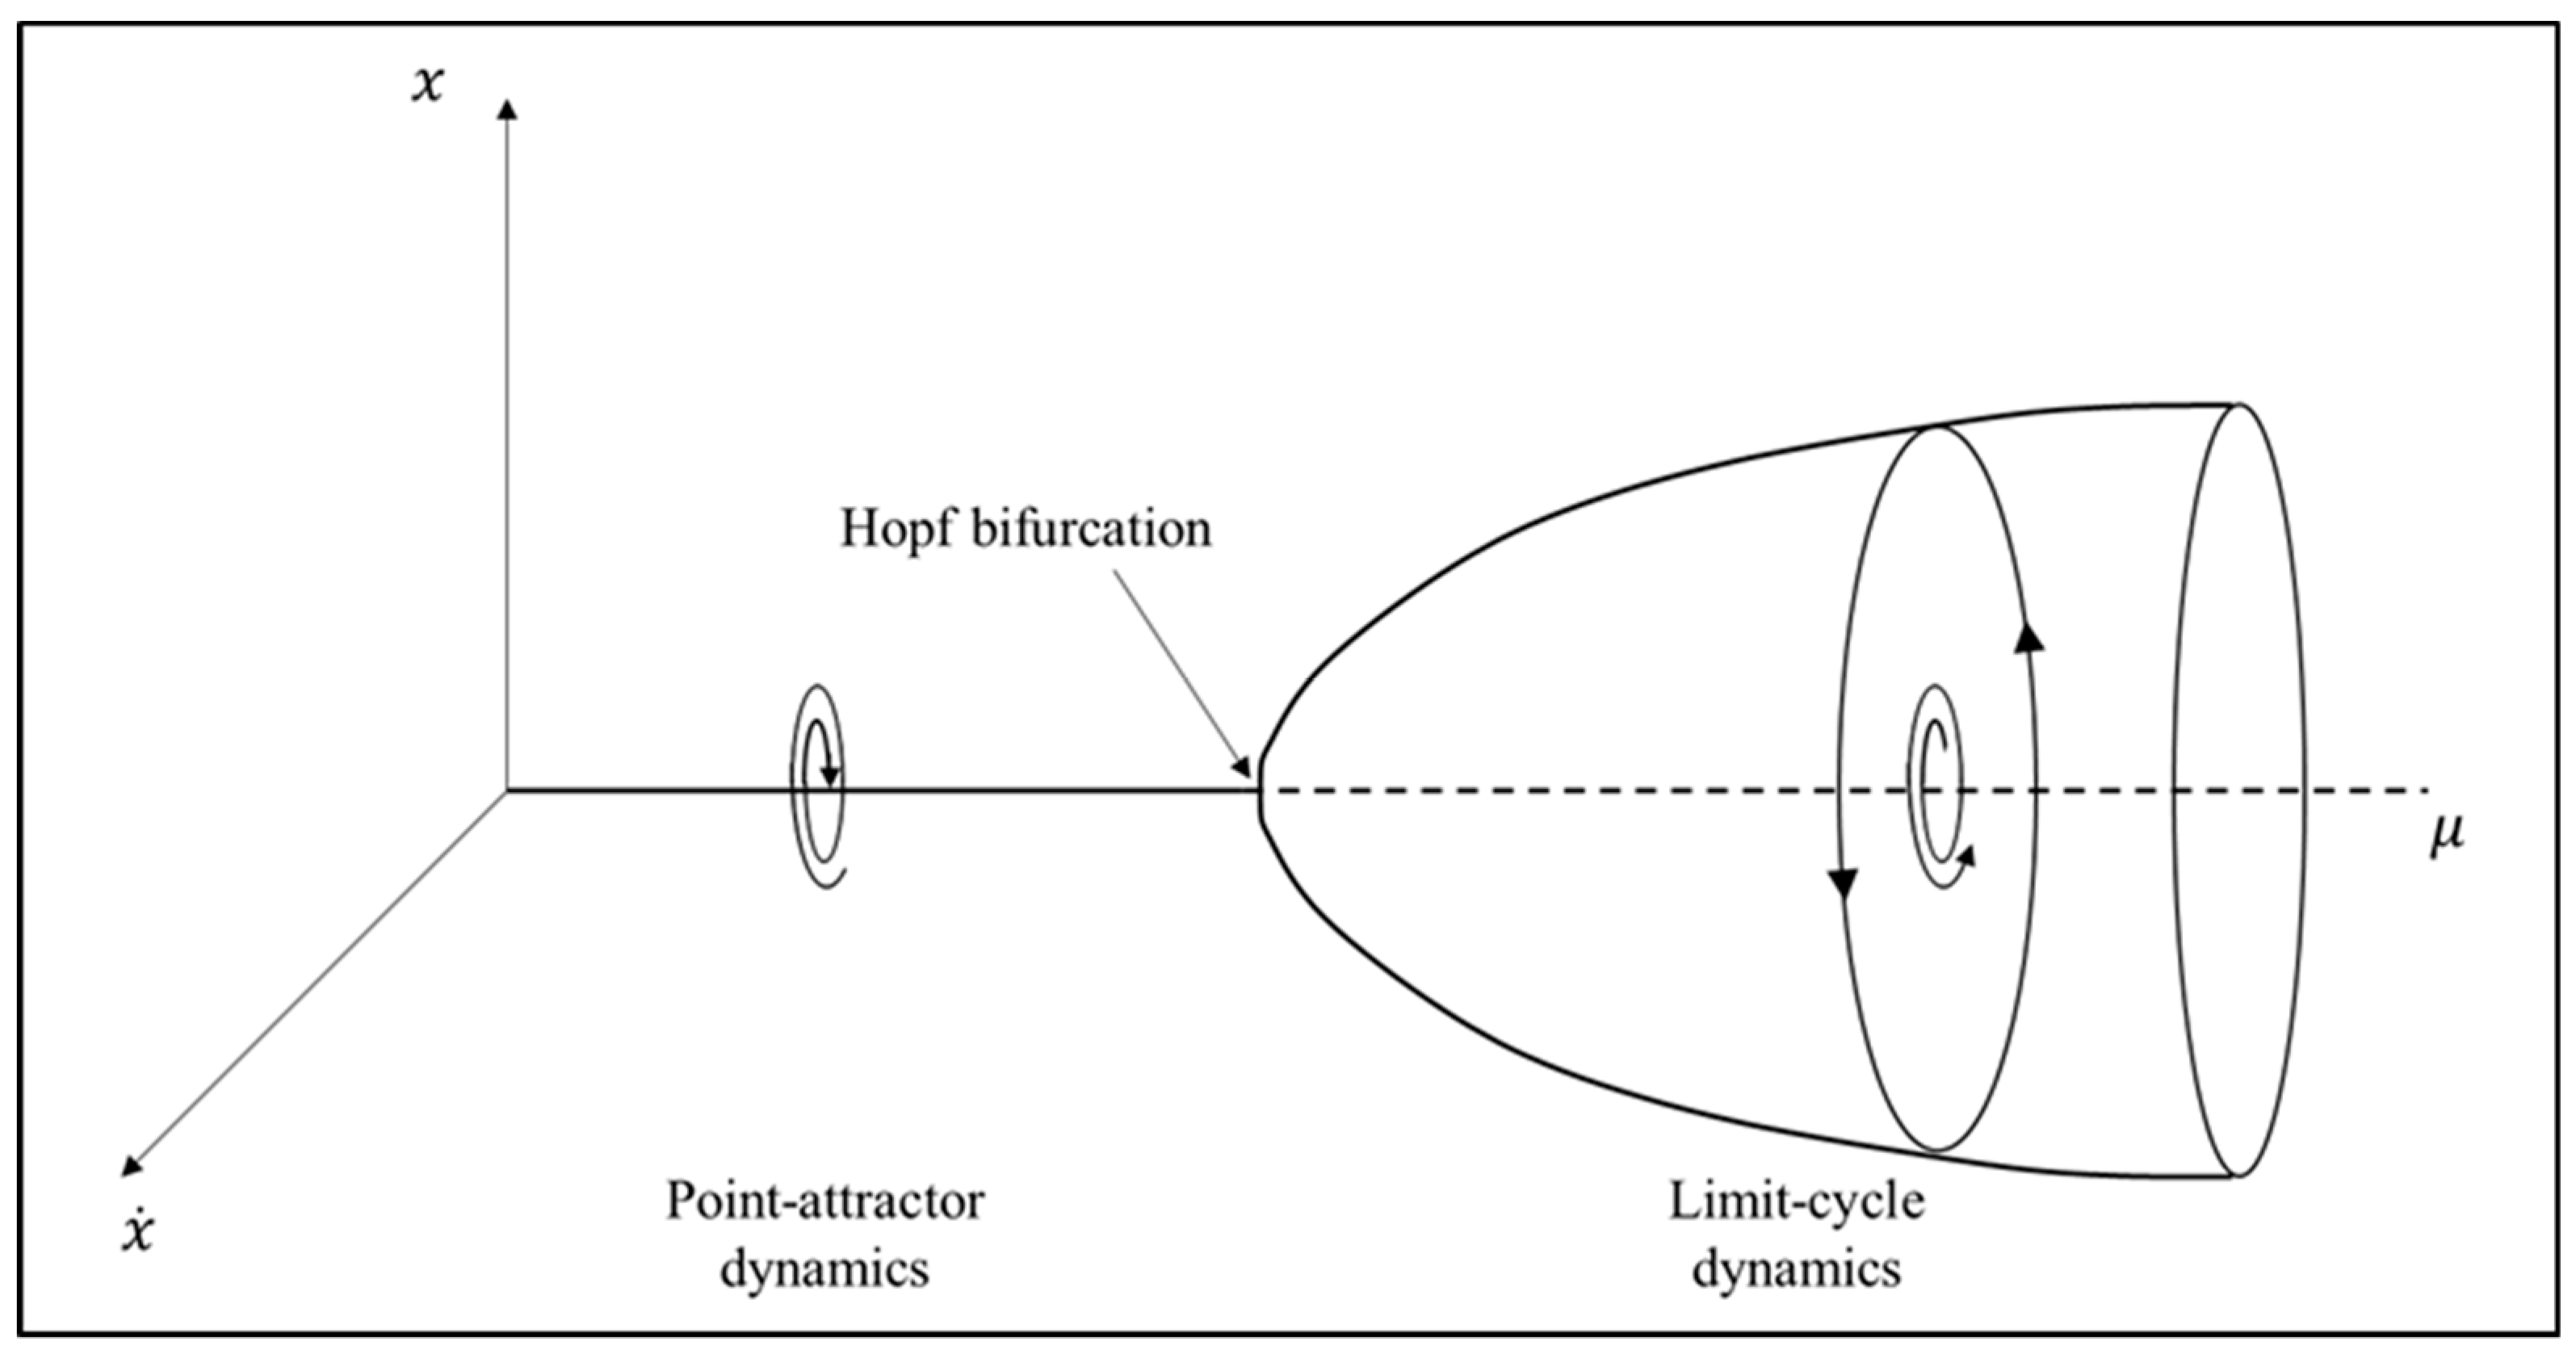
\includegraphics[width=0.8\linewidth]{pics/hopf-bif-pic.png}\\
	\tiny (Illustrative: Hopf vs Pitchfork bifurcations)
\end{frame}

\begin{frame}
	\centering
	
\includegraphics[width=0.54\linewidth]{pics/leo.jpg}
\end{frame}

\begin{frame}
	\centering
	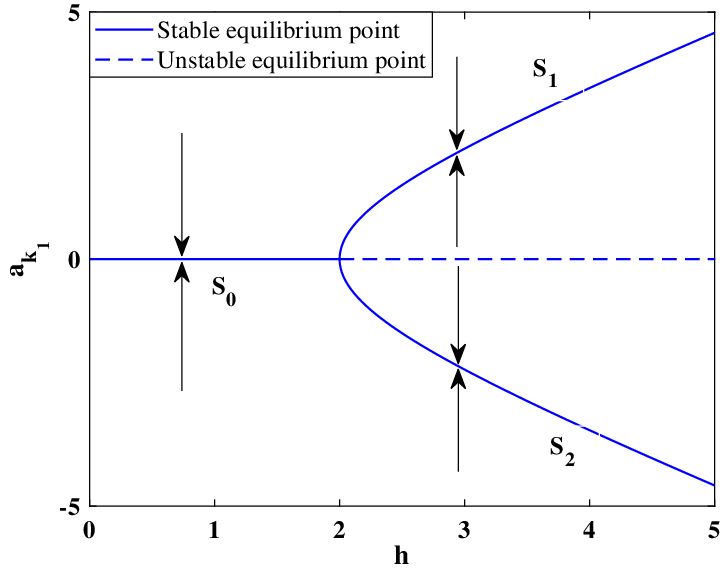
\includegraphics[width=0.7\linewidth]{pics/pitchfork-photo.png}
\end{frame}

% --- Section 5: Detecting Hopf Bifurcations ---
\section{Detecting Hopf Bifurcations}

\begin{frame}{\insertsectionhead}
	\frametitle{Characteristic Polynomial \& Routh-Hurwitz}
	\begin{itemize}
		\item Characteristic polynomial of $J(\mu)$:
			$$ P(\lambda, \mu) = \det(J(\mu) - \lambda I_n) = a_0\lambda^n + a_1\lambda^{n-1} + \dots + a_n = 0 $$
			(Assume $a_0 > 0$, coefficients $a_i$ depend on $\mu$).
		\item \alert{Routh-Hurwitz criterion}: Conditions on $a_i(\mu)$ for all Re($\lambda_k$) $< 0$.
		\item Involves \alert{Hurwitz matrices} $H_k(\mu)$. For $n$, $H_n(\mu)$:
			$$  H_n(\mu) =
			\begin{pmatrix}
				a_1 & a_3 & a_5 & \dots \\
				a_0 & a_2 & a_4 & \dots \\
				0 & a_1 & a_3 & \dots \\
				\vdots & \vdots & \ddots & \vdots \\
				0 & \dots & & a_n
			\end{pmatrix}
			= (a_{2j - i})_{ij}$$
			($a_k = 0$ if $k<0$ or $k>n$).
		\item Stability $\iff$ all leading principal minors $\Delta_k = \det H_k(\mu)$ are positive: $\det H_i(\mu) > 0, \forall i = \overline{1,n}$.
	\end{itemize}
\end{frame}

\begin{frame}{\insertsectionhead}
	\frametitle{Criterion for Hopf Bifurcation (Yang)}
	For a system of effective degree $s \ge 2$ (after factoring out zero eigenvalues), a simple Hopf bifurcation occurs at $\mu_0$ if:
	\begin{enumerate}
		\item $\det H_{s-1}(\mu_0) = 0$.
		\item $\det H_1(\mu_0) > 0, \dots, \det H_{s-2}(\mu_0) > 0$.
		\item $a_s(\mu_0) > 0$ (constant term of the effective characteristic polynomial).
		\item Transversality: $\frac{d}{d\mu}(\det H_{s-1}(\mu))\bigg|_{\mu_0} \neq 0$.
	\end{enumerate}
	These ensure one pair of purely imaginary eigenvalues crosses the axis, others stable.
\end{frame}

\begin{frame}{\insertsectionhead}
	\frametitle{(Thm.) Ruling Out Hopf Bifurcations}
	No simple Hopf bifurcation along $x^*(\mu)$ if, for all relevant $\mu$:
	\begin{itemize}
		\item $\det H_1(\mu) > 0, \dots, \det H_{s-2}(\mu) > 0$ (preliminary stability for other roots),
		\item AND either:
			\begin{itemize}
				\item Whenever $\det H_{s-1}(\mu) = 0 \implies a_s(\mu) \le 0$. (breaks condition 3)
				\item OR, $\det H_{s-1}(\mu) \neq 0$ for all $\mu$. (breaks condition 1)
			\end{itemize}
	\end{itemize}
	The system never meets the precise criteria for a Hopf bifurcation.
\end{frame}

% --- Section 6: Application to (De)phosphorylation CRNs ---
\section{Application to (De)phosphorylation CRNs}

\begin{frame}{\insertsectionhead}
	\frametitle{(De)phosphorylation Cycles: Cellular Switches \& Clocks}
	\begin{itemize}
		\item (De)phosphorylation cycles are key in \alert{signal transduction}.
		\item Involve: Substrate $S$ (forms $S_0, \dots, S_n$), Kinase $K$, Phosphatase $F$.
		\item Example (single site) $\mathcal{N}_1$:
			\begin{align*}
				S_0 + K &\rightleftharpoons KS_0 \xrightarrow{k_3} S_1 + K \\
				S_1 + F &\rightleftharpoons FS_1 \xrightarrow{k_6} S_0 + F
			\end{align*}
		\item \alert{Key Question}: Can these networks act as \alert{switches} (multiple steady states, bistability) or as \alert{clocks} (sustained oscillations via Hopf)? This determines their functional role.
	\end{itemize}
\end{frame}

\begin{frame}
	% picture insert
	\centering
	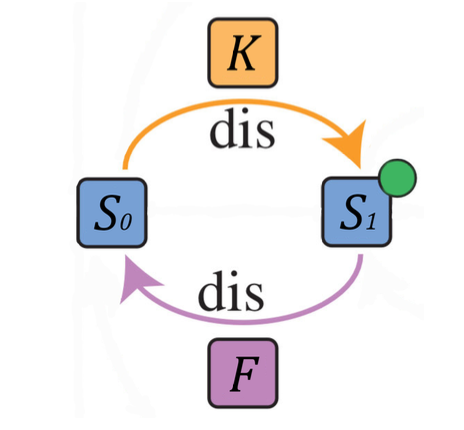
\includegraphics[width=0.5\linewidth]{pics/ex1-no-bifurcations.png} \\ 	

	\begin{align*}
		S_0 + K &\rightleftharpoons KS_0 \xrightarrow{k_3} S_1 + K  \tag{$\mathcal{N}_1$} \\
		S_1 + F &\rightleftharpoons FS_1 \xrightarrow{k_6} S_0 + F
	\end{align*}
\end{frame}

\begin{frame}{\insertsectionhead}
	\frametitle{Types of (De)phosphorylation Mechanisms}
	The specific mechanism influences dynamic behavior:
	\begin{itemize}
		\item \alert{Distributive}: Enzyme dissociates after each single modification event.
			\begin{itemize}
				\item $S_0 + K \to \dots \to S_1 + K$, then $S_1 + K \to \dots \to S_2 + K$.
			\end{itemize}
		\item \alert{Processive}: Enzyme performs multiple modifications before dissociating.
			\begin{itemize}
				\item $S_0 + K \to S_0K \to S_1K \to \dots \to S_n + K$.
			\end{itemize}
		\item For multi-site phosphorylation (e.g., two sites $S_{ij}$):
			\begin{itemize}
				\item \alert{Sequential}: Last site phosphorylated is first dephosphorylated (e.g., $S_{00} \to S_{10} \to S_{11} \to S_{01} \to S_{00}$).
				\item \alert{Cyclic (ordered)}: First site phosphorylated is first dephosphorylated (e.g., $S_{00} \to S_{10} \to S_{11} \to S_{10 \text{ (F removes from site 1)}} \to S_{00 \text{ (F removes from site 0)}}$ - this is a common depiction but the example from `main.pdf` for N2 is $S_{00} \leftrightarrow S_{10} \leftrightarrow S_{11} \leftrightarrow S_{01} \leftrightarrow S_{00}$).
			\end{itemize}
	\end{itemize}
	\centering
	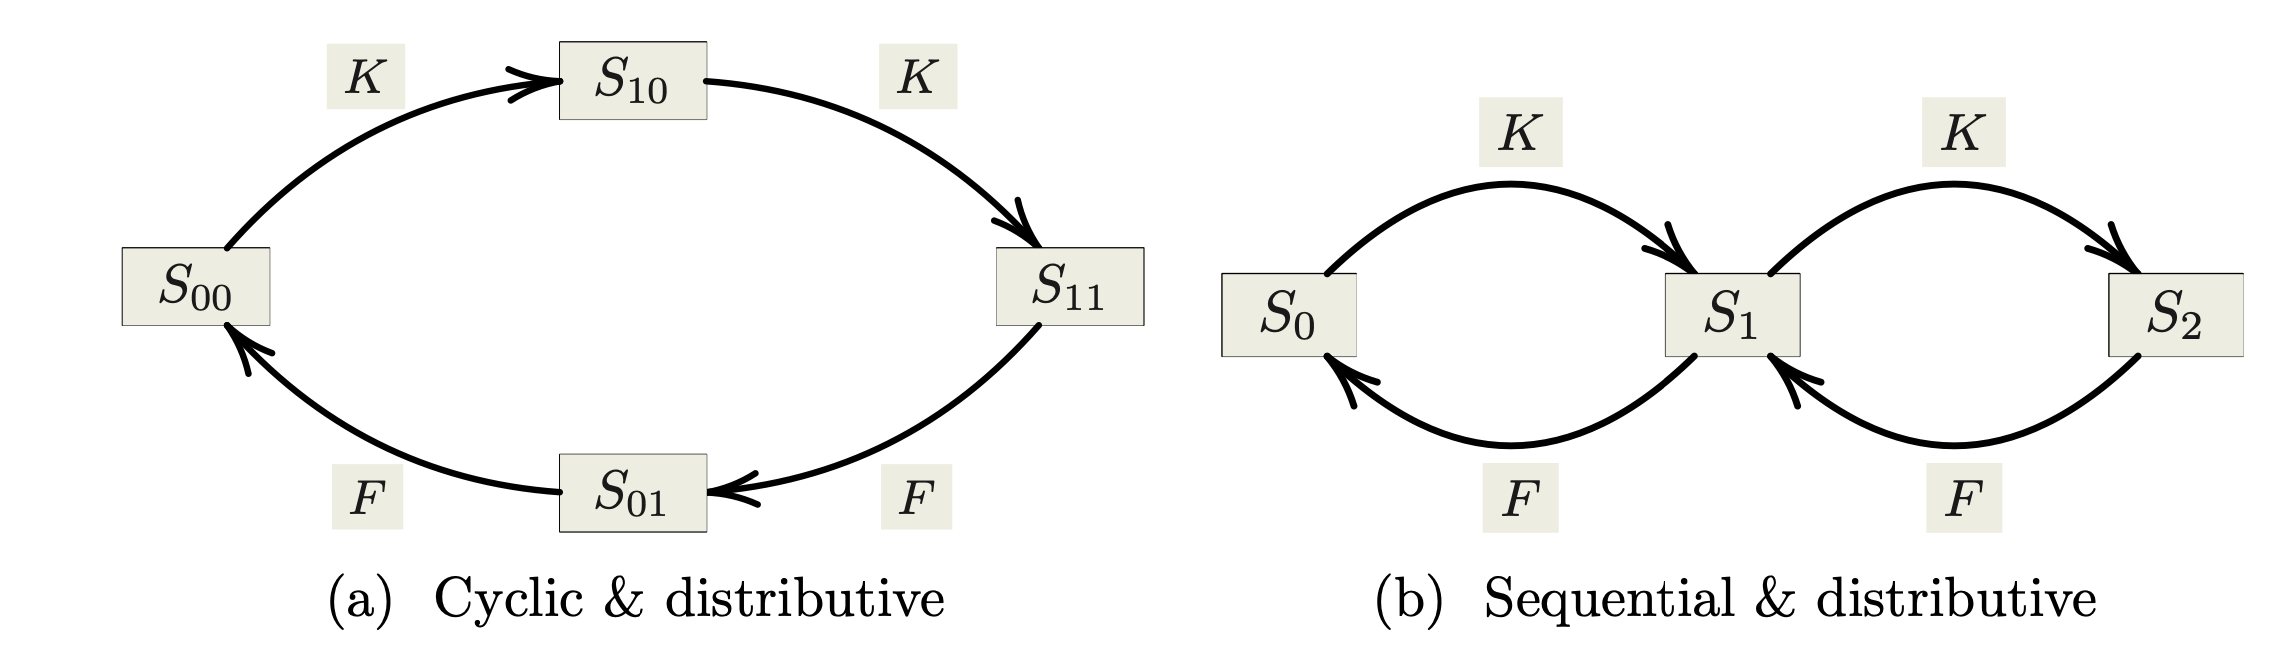
\includegraphics[width=0.6\linewidth]{pics/cyclic-vs-sequential.png} \\
	\tiny (Illustrative: Placeholder for Fig (a) and (b) from `main.pdf` section 4.3.1)
\end{frame}

\begin{frame}{\insertsectionhead}
	\frametitle{Convex Parameters for CRN Analysis}
	\begin{itemize}
		\item Jacobian $J(k, x^*)$ analysis can be algebraically complex.
		\item \alert{Convex parameterization} $(h, \lambda)$ can simplify $J$:
			\begin{itemize}
				\item $h_i = \frac{1}{x_i^*}$ (inverse steady-state concentrations).
				\item $v^* = E\lambda$ : flux vector, $E$ matrix of extreme rays of flux cone $\text{ker}(\Gamma) \bigcap \mathbb{R}^r_{\ge 0}$, $\lambda$ convex parameters.
				\item $J(h, \lambda) = \Gamma \text{diag}(E\lambda) \Gamma_L^T \text{diag}(h)$ (cool trick that differentiates).
			\end{itemize}
		\item Coefficients of $J(h,\lambda)$ become \alert{monomials} in $h, \lambda$, simplifying analysis of Hurwitz determinants.
	\end{itemize}
\end{frame}

\begin{frame}{\insertsectionhead}
	\frametitle{Simplification: Single Extreme Ray Case}
	If the steady-state flux cone is a single ray ($l=1$, $v^* = \lambda_1 E_1$):
	\begin{itemize}
		\item Jacobian: $J_{\lambda_1}(h) = \lambda_1 (\Gamma \text{diag}(E_1) \Gamma_L^T \text{diag}(h)) = \lambda_1 J_1(h)$.
		\item Eigenvalues: $\text{eig}(J_{\lambda_1}(h)) = \lambda_1 \cdot \text{eig}(J_1(h))$.
			\begin{itemize}
				\item Sign of real parts is preserved.
				\item Purely imaginary eigenvalues $\pm i \omega_0$ for $J_1(h)$ become $\pm i \lambda_1 \omega_0$ for $J_{\lambda_1}(h)$.
			\end{itemize}
		\item Characteristic polynomial coefficients: $a_i(\lambda_1, h) = \lambda_1^i b_i(h)$, where $b_i(h)$ are for $J_1(h)$.
		\item Hurwitz determinants: $\det(H_k(\lambda_1,h)) = \lambda_1^{k(k+1)/2} \det(G_k(h))$, where $G_k(h)$ are for $J_1(h)$.
		\item \alert{Hopf analysis depends primarily on $h$ (via $b_i(h)$ and $G_k(h)$), not $\lambda_1$ as a bifurcation parameter for crossing.}
	\end{itemize}
\end{frame}

\begin{frame}{\insertsectionhead}
	\frametitle{Example 1: Network $\mathcal{N}_1$ (Basic Cycle)} Using this as example I'll also showcase \href{https://github.com/viktorashi/Open-CoNtRol}{the app} that I've been working on for my thesis.
	For $K + S_0 \rightleftharpoons KS_0 \rightarrow K + S_1$, $F + S_1 \rightleftharpoons FS_1 \rightarrow F + S_0$ ($\mathcal{N}_1$):
	\begin{align*}
		\Gamma &=
		\begin{pmatrix}
			K & -1 &  1 &  1 &  0 &  0 &  0 \\
			S0& -1 &  1 &  0 &  0 &  0 &  1 \\
			KS0 &  1& -1& -1 &  0 &  0 &  0 \\
			S1 &  0 &  0 &  1& -1 &  1 &  0 \\
			F &  0 &  0 &  0& -1 &  1 &  1 \\
			FS1 &  0 &  0 &  0 &  1& -1& -1  \\		
		\end{pmatrix}, \quad \text{rank}(\Gamma) = 3 \\[3ex]
		\Gamma_L &=
		\begin{bmatrix}
			1&0&0&0&0&0\\
			1&0&0&0&0&0\\
			0&1&1&0&0&0\\
			0&0&0&1&0&0\\
			0&0&0&1&0&0\\
			0&0&0&0&1&1
		\end{bmatrix} \\[3ex]
	\end{align*}
\end{frame}

\begin{frame}
	\begin{align*}
		\begin{cases*}
			\begin{array}{ll}
				\dot{x}_1(t) = -k_4 x_1(t) *x_6(t)+k_5 x_2(t)+k_6 x_2(t) \\
				\dot{x}_2(t) = k_4 x_1(t) *x_6(t)-k_5 x_2(t)-k_6 x_2(t) \\
				\dot{x}_3(t) = -k_1 x_3(t) *x_5(t)+k_2 x_4(t)+k_3 x_4(t) \\
				\dot{x}_4(t) = k_1 x_3(t) *x_5(t)-k_2 x_4(t)-k_3 x_4(t) \\
				\dot{x}_5(t) = -k_1 x_3(t) *x_5(t)+k_2 x_4(t)+k_6 x_2(t) \\
				\dot{x}_6(t) = k_3 x_4(t)-k_4 x_1(t) *x_6(t)+k_5 x_2(t) \\
			\end{array}	
		\end{cases*}		
	\end{align*}
	is the output it generated.
	Where the "species to index mapping" is:
	\[
		F:  x_1
		| FS1: x_2
		| K: x_3
		| KS0: x_4
		| S0: x_5
		| S1: x_6
	\]
	\textbf{Remark 1:} $(a)$ As you can see, ($\mathcal{N}_1$) consists of $6$ species ($2$ substrates $S_0$, $S_1$; $2$ enzymes $K$, $F$; which together form $2$ complexes: $K S_0$, $F S_1$) and $6$ reactions ($2$ reversible and $2$ irreversible) with matrix subspace $=$ rank $\Gamma = 3$.
\end{frame}

\begin{frame}
	\begin{itemize}
		\item \textbf{Remark 1:} $(b)$ For ($\mathcal{N}_1$), the cone $\Gamma v(k,x) = 0, \forall v \geqq 0$ is spanned by the vectors $w_0, w_1, w_2 \geqq 0 : \lambda_0 w_0 + \lambda_1 w_1 + \lambda_2 w_2 \geqq 0 \iff \lambda_1, \lambda_2, \lambda_3 \geq 0$.	
			$E\lambda$ matrix made of the extreme cone vectors (\textbf{ray}):
			\[
				E\lambda =
				\begin{bmatrix}
					\lambda_2 + \lambda_3 \\
					\lambda_1 \\
					\lambda_3 \\
					\lambda_2 + \lambda_3 \\
					\lambda_2 \\
					\lambda_3
				\end{bmatrix}
			\]
		\item Now we may consider the Jacobian written in convex parameters for $\mathcal{N}_1$, $J_1(h,\lambda)$, which is parametrized by $9$ parameters: $\lambda_0, \lambda_1, \lambda_2$ and $h_1, \ldots, h_6$.
	\end{itemize}
\end{frame}

\begin{frame}
	\[
		\left. J_1(h, \lambda) =\left[
			\begin{array}{ccccccc}-\lambda_1hl&-\lambda_1h2&0&0&0&0&\lambda_1h7\\-\lambda_1hl&-\lambda_1h2&\lambda_1h3&0&0&0&0\\\lambda_1hl&\lambda_1h2&-\lambda_1h3&0&0&0&0\\0&-\lambda_2h2&\lambda_1h3&(-\lambda_2-\lambda_1)h4&0&\lambda_2h6&0\\0&\lambda_2h2&0&\lambda_2h4&-\lambda_2h5&0&0\\0&0&0&0&\lambda_2h5&-\lambda_2h6&0\\0&0&0&\lambda_1h4&0&0&-\lambda_1h7
		\end{array}\right.\right]
	\]
\end{frame}

\begin{frame}
	\begin{itemize}
		\item So, from \textbf{Remark 1} $(a)$ and $(b)$, it follows that the characteristic polynomial of $J_1(h, \lambda)$ is
			\[
				p_{h,\lambda}(z) = z^3 (a_0(h,\lambda) z^3 + a_1(h,\lambda) z^2 + a_2(h,\lambda) z + a_3(h,\lambda))
			\]
			Whose Hurwitz is pretty huge (will always overflow \TeX).
	\end{itemize}
	But do trust me that:
	\begin{itemize}
		\item Effective degree $s=3$. Critical Hurwitz determinant is $\det H_2(h,\lambda)$.
		\item Analysis shows for $\mathcal{N}_1$:
			$\det H_1(h, \lambda) > 0$, $\det H_2(h, \lambda) > 0$, $a_3(h, \lambda) > 0$, meaning
		\item $a_3(k, x^*) > 0$ (highest degree polynomial coefficient)
		\item Since $\det H_2(h, \lambda)$ is always positive (sum of positive monomials)
		\item \alert{Conclusion}: Network $\mathcal{N}_1$ does not admit simple Hopf bifurcations.
	\end{itemize}
\end{frame}

% --- Section 7: Case Study: Network N2 - Finding Oscillations ---
\section{Case Study: Network N2 - Finding Oscillations}

\begin{frame}{\insertsectionhead}
	\frametitle{Network $\mathcal{N}_2$: A Cyclic Double Phosphorylation System}
	Consider the cyclic, distributive double (de)phosphorylation system
	\centering
	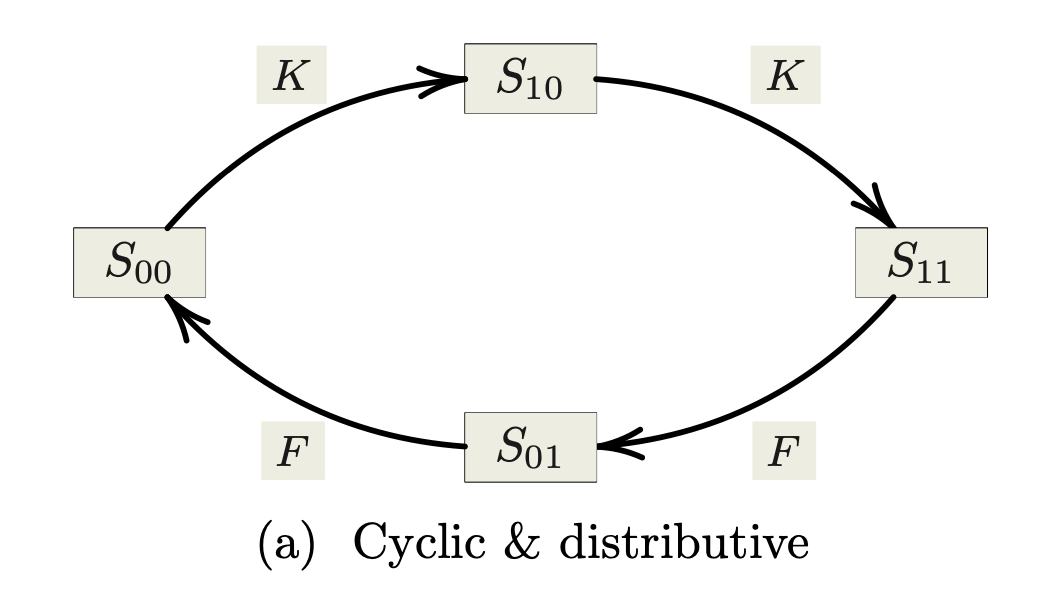
\includegraphics[width=0.6\linewidth]{pics/cyclic-distributive-n1.png} \\
	\begin{align*}
		S_{00} + K &\rightleftharpoons KS_{00} \rightarrow S_{10} + K & S_{10} + K &\rightleftharpoons KS_{10} \rightarrow S_{11} + K \tag{$\mathcal{N}_2$} \\
		S_{11} + F &\rightleftharpoons FS_{11} \rightarrow S_{01} + F & S_{01} + F &\rightleftharpoons FS_{01} \rightarrow S_{00} + F
	\end{align*}
	We analyze its \alert{irreversible version} for Hopf bifurcations.
\end{frame}

\begin{frame}{\insertsectionhead}
	\frametitle{$\mathcal{N}_3$ (Irreversible): Setup for Analysis}
	Irreversible reactions:
	\begin{align*}
		S_{00} + K \xrightarrow{\kappa_1} KS_{00} \xrightarrow{\kappa_3} S_{10} + K \xrightarrow{\kappa_4} KS_{10} \xrightarrow{\kappa_6} S_{11} + K \tag{$\mathcal{N}_3$}
		\\
		S_{11} + F \xrightarrow{\kappa_7} FS_{11} \xrightarrow{\kappa_9} S_{01} + F \xrightarrow{\kappa_{10}} FS_{01} \xrightarrow{\kappa_{12}} S_{00} + F \ \notag
	\end{align*}
	\begin{itemize}
		\item 10 species, 8 reactions.
		\item 3 conservation laws (total kinase, total phosphatase, total substrate) $\implies$ rank of Jacobian is $10-3=7$. So, effective degree $s=7$.
		\item The steady-state flux cone is a \alert{single extreme ray} $E^T = (1,1,1,1,1,1,1,1)$.
		\item We can use the $J_\lambda(h) = \lambda J_1(h)$ simplification.
	\end{itemize}
\end{frame}

\begin{frame}
	\[
		\begin{aligned}
			\dot{x}_{1} &= -\kappa_{1} x_{1} x_{3} - \kappa_{4} x_{1} x_{4} + \kappa_{3} x_{7} + \kappa_{6} x_{8},\\
			\dot{x}_{2} &= \kappa_{9} x_{10} - \kappa_{10} x_{2} x_{5} - \kappa_{7} x_{2} x_{6} + \kappa_{12} x_{9},\\
			\dot{x}_{3} &= -\kappa_{1} x_{1} x_{3} + \kappa_{12} x_{9},\\
			\dot{x}_{4} &= -\kappa_{4} x_{1} x_{4} + \kappa_{3} x_{7},\\
			\dot{x}_{5} &= \kappa_{9} x_{10} - \kappa_{10} x_{2} x_{5},\\
			\dot{x}_{6} &= -\kappa_{7} x_{2} x_{6} + \kappa_{6} x_{8},\\
			\dot{x}_{7} &= \kappa_{1} x_{1} x_{3} - \kappa_{3} x_{7},\\
			\dot{x}_{8} &= \kappa_{4} x_{1} x_{4} - \kappa_{6} x_{8},\\
			\dot{x}_{9} &= \kappa_{10} x_{2} x_{5} - \kappa_{12} x_{9},\\
			\dot{x}_{10} &= -\kappa_{9} x_{10} + \kappa_{7} x_{2} x_{6}.
		\end{aligned}
	\]
	Now there are 3 conservation laws for both networks, diminishing the rank of the Jacobian matrix to $7$. These are:
	\[
		\begin{aligned}
			x_{1}+x_{7}+x_{8}&=c_{1}\\x_{2}+x_{9}+x_{10}&=c_{2}\\x_{3}+x_{4}+x_{5}+x_{6}+x_{7}+x_{8}+x_{9}+x_{10}&=c_{3}
		\end{aligned}
	\]
\end{frame}

\begin{frame}
	And Now with the simplifications we can obtain the relations
	\begin{gather*}
		\kappa_1x_1x_3=\kappa_3x_7=\kappa_4x_1x_4=\kappa_6x_8=\kappa_7x_2x_6=\kappa_9x_{10}=\kappa_{10}x_2x_5=\kappa_{12}x_9=\lambda. \\
		\Downarrow \\
		x_{3} = \frac{\lambda}{\kappa_{1} x_{1}}, \ x_{4} = \frac{\lambda}{\kappa_{4} x_{1}}, \ x_{5} = \frac{\lambda}{\kappa_{10} x_{2}}, \ x_{6} = \frac{\lambda}{\kappa_{7} x_{2}} \\
		x_{7} = \frac{\lambda}{\kappa_{3}}, \ x_{8} = \frac{\lambda}{\kappa_{6}}, \ x_{9} = \frac{\lambda}{\kappa_{12}}, \ x_{10} = \frac{\lambda}{\kappa_{9}} \\
		\forall x_1, x_2 > 0 \\
		\Downarrow \\
		\kappa_{1} = h_{1} h_{3} \lambda, \kappa_{3} = h_{7} \lambda, \kappa_{4} = h_{1} h_{4} \lambda, \kappa_{6} = h_{8} \lambda \\
		\kappa_{7} = h_{2} h_{6} \lambda, \kappa_{9} = h_{10} \lambda, \kappa_{10} = h_{2} h_{5} \lambda, \kappa_{12} = h_{9} \lambda \\
		\text{with } h_i = \frac{1}{x_i} , i = \overline{1,10}
	\end{gather*}
\end{frame}

\begin{frame}
	And, $J_\lambda(h)$:
	\begin{align}
		J_\lambda(h) = \lambda
		\left.\left[
			\begin{array}{rrrrrrrrrr}-2h_{1}&0&-h_{3}&-h_{4}&0&0&h_{7}&h_{3}&0&0\\0&-2h_{2}&0&0&-h_{5}&-h_{6}&0&0&h_{9}&h_{10}\\-h_{1}&0&-h_{3}&0&0&0&0&0&h_{3}&0\\-h_{1}&0&0&-h_{4}&0&0&h_{7}&0&0&0\\0&-h_{2}&0&0&-h_{5}&0&0&0&0&h_{10}\\0&-h_{2}&0&0&0&-h_{6}&0&h_{3}&0&0\\h_{1}&0&h_{3}&0&0&0&-h_{7}&0&0&0\\h_{1}&0&0&h_{4}&0&0&0&-h_{3}&0&0\\0&h_{2}&0&0&h_{5}&0&0&0&-h_{9}&0\\0&h_{2}&0&0&0&0&h_{6}&0&0&-h_{10}
		\end{array}\right.\right]
	\end{align}
	with $rank(J_\lambda(h)) = 7$ and characteristic polynomial is of the form:
	\[
		\det\left(\mu I-J_\lambda(h)\right)=\mu^3\left(\mu^7+\lambda b_1(h)\mu^6+\ldots+\lambda^6b_6(h)\mu+\lambda^7b_7(h)\right),
	\]
	With $b_i(h)$ from char. poly of $J_1(h)$.
\end{frame}

\begin{frame}
	Now, constructing the (simplified) Hurwitz matrices $G_i(h), i = \overline{1,6}$. Assume that at a fixed $h = h^*$ the following occur.
	\[
		\begin{aligned}b_{7}(h^{*})&>0and\\\det(G_1(h^*))&>0,\ldots,\det(G_5(h^*))>0and\\\det(G_6(h^*))&=0.
		\end{aligned}
	\]
	then, if additionally:
	\[
		\exists l\in\{1,\ldots,10\} : \frac{\partial\det(G_6)}{\partial h_l}|_{h=h^*}\neq0\quad.
	\]

	Then ($\mathcal{N}_3$) has a simple Hopf bifurcation at $h = h^*, \forall \lambda > 0$.

	$\det(G_6(h))$ has terms with both signs (trust me), so it may have roots.

	In the following section we'll talk about $\det(G_6(h))$'s potential to have roots.
\end{frame}

\begin{frame}
	\frametitle{Polytopes}
	First (and I swear this is relevant), let's look at some shapes:

	These are all (k)-\textbf{polytopes}, shapes whose faces are flat (k-1)-\textbf{polytopes}.
	\begin{figure}[H]
		\centering
		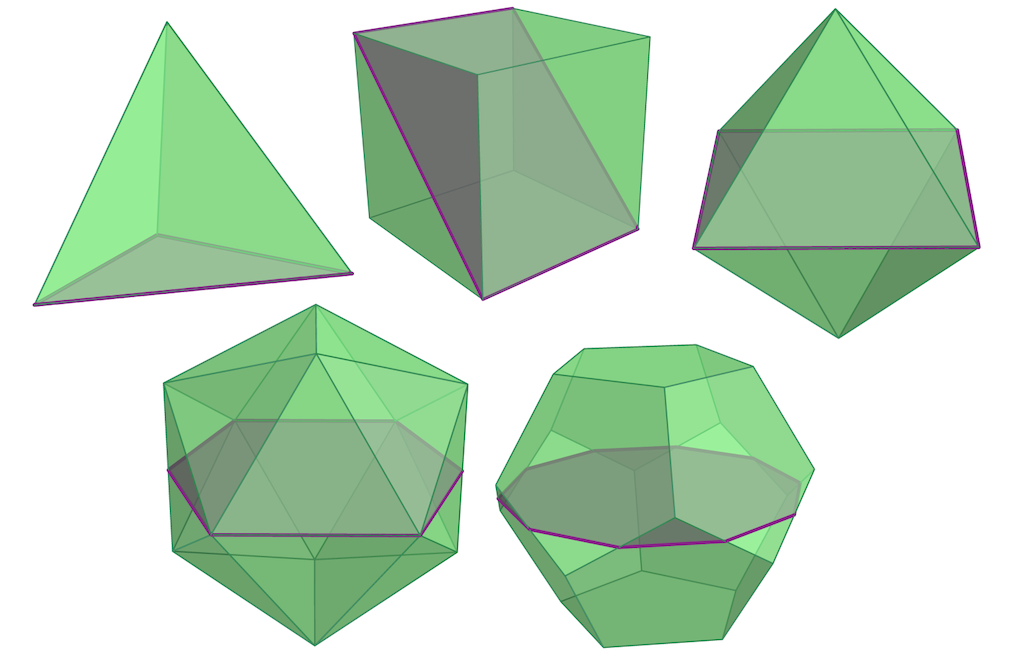
\includegraphics[width=0.5\linewidth]{pics/polytopes.png}
		\caption{Polytopes}
	\end{figure}
\end{frame}

\begin{frame}
	The \textbf{Newton polytope} of that polynomial is.
	\[
		\mathrm{Newt}(f)=\left\{\sum_k\alpha_k\mathbf{a}_k:\sum_k\alpha_k=1 \And \forall j\alpha_j\geq0\right\}. \forall c_k \neq 0_n
	\]a structure that offers insight into the coefficients.
	Using a software like \href{https://polymake.org/doku.php/start}{Polymake} we're able to observe that the factor $	h_{10}h_7 - h_8 h_9$ appears in the hyper-plane representation of the polytope, which is of help to us since it has negative factors.
	Doing the restriction / transformation $	h_1\to t,h_2\to t,h_3\to t,h_6\to t.$ We're able to represent $\det G_6(h)$ as:
	\[
		\begin{aligned}
			\det G_6(t)
			&=324t^{18}(h_{10}+h_7)(h_{10}h_7-h_8h_9)+\ldots\\&+h_{10}h_4h_5h_7h_8h_9\\&\cdot(h_{10}+h_4)(h_{10}+h_5)(h_{10}+h_7)(h_{10}+h_8)(h_{10}+h_9)\\&\cdot(h_4+h_5)(h_4+h_7)(h_4+h_8)(h_4+h_9)\\&\cdot(h_5+h_7)(h_5+h_8)(h_5+h_9)\\&\cdot(h_7+h_8)(h_7+h_9)\\&\cdot(h_8+h_9).
		\end{aligned}
	\]
\end{frame}

\begin{frame}{\insertsectionhead}
	\frametitle{$\mathcal{N}_3$: Transversality}
	$\det G_6(0) > 0$, so if $h_{10}h_{7} - h_{8}h_{9} < 0, \implies \exists t_1 > 0 : \det G_6(t_1) = 0, \det G_6(t) < 0, \forall t > t_1$ by the \alert{Intermediate Value Theorem}.
	So it means we've shown a root exists for $\det G_6(h)$, so a bifurcation may occur in our system.

	Once a root $h^*$ for $\det G_6(h)=0$ is found (with other Hurwitz determinants positive), the transversality condition must also be checked:
	$$ \frac{\partial \det(G_6(h))}{\partial h_l} \bigg|_{h=h^*} \neq 0 \quad \text{for some } l \in \{1, \dots, 10\} $$
	This ensures the eigenvalues genuinely cross the imaginary axis.
\end{frame}

\begin{frame}
	\frametitle{$\mathcal{N}_3$: Conclusion}
	\begin{itemize}
		\item Calculations (often symbolic and extensive) can confirm this for specific parameter regions.
		\item \alert{Conclusion for $\mathcal{N}_2$}: The cyclic double (de)phosphorylation network $\mathcal{N}_2$ (irreversible version) \alert{can exhibit simple Hopf bifurcations} for certain parameter values $h^*$ (and any $\lambda > 0$).
		\item This means this network structure is capable of generating sustained oscillations, acting as a biochemical clock.
	\end{itemize}
\end{frame}

% --- Section 8: Conclusion ---
\section{Conclusion}

\begin{frame}{\insertsectionhead}
	\frametitle{Summary: Unveiling Chemical Rhythms}
	\begin{itemize}
		\item Hopf bifurcations are critical for understanding how \alert{oscillations} arise in CRNs.
		\item This is vital for (de)phosphorylation networks, which underpin cellular signaling and control.
		\item Proving existence/absence of Hopf involves:
			\begin{enumerate}
				\item ODE model $\to$ Equilibria $\to$ Jacobian $J$.
				\item Characteristic polynomial of $J$.
				\item Routh-Hurwitz determinants ($\Delta_k$) to check stability and Hopf conditions (esp. $\Delta_{s-1}=0$, $\Delta_{s-2}>0, \dots, \Delta_1>0, a_s>0$, transversality).
			\end{enumerate}
		\item \alert{Convex parameterization} and \alert{single extreme ray} analysis can greatly simplify complex CRNs.
		\item We saw Network $\mathcal{N}_1$ (basic cycle) \alert{cannot} have Hopf bifurcations.
		\item We saw Network $\mathcal{N}_2$ (cyclic double phosphorylation) \alert{can} have Hopf bifurcations (shown through polytope tricks), providing a mechanism for intrinsic oscillations while showcasing some functions of the web-application.
		\item This mathematical framework allows rigorous investigation of biological "clocks" and "switches".
	\end{itemize}
\end{frame}

\begin{frame}[plain]
	\centering
	\vfill
	\Huge Thank You!
	\vfill
	Questions? \\
	{\small (please don't) }
	\vfill
\end{frame}

\end{document}
